\chapter{Arquitectura de un robot delta}\label{CAP3}

\section{Funcionamiento general}

La principal tarea de un robot es ir de un punto a otro para realizar determinada acción. Para realizar la tarea se debe pasar por una serie de pasos con el fin de asegurar la ejecución exitosa de dicha tarea. Con el fin de explicar brevemente los pasos a seguir para lograr dicho objetivo, en la figura \ref{f:Cap3-1_diagrama_de_flujo_robot_accion} se muestra un ejemplo básico de un diagrama de flujo de un robot delta accionado por motores paso a paso.

    \begin{figure}[htb]
        \centering
        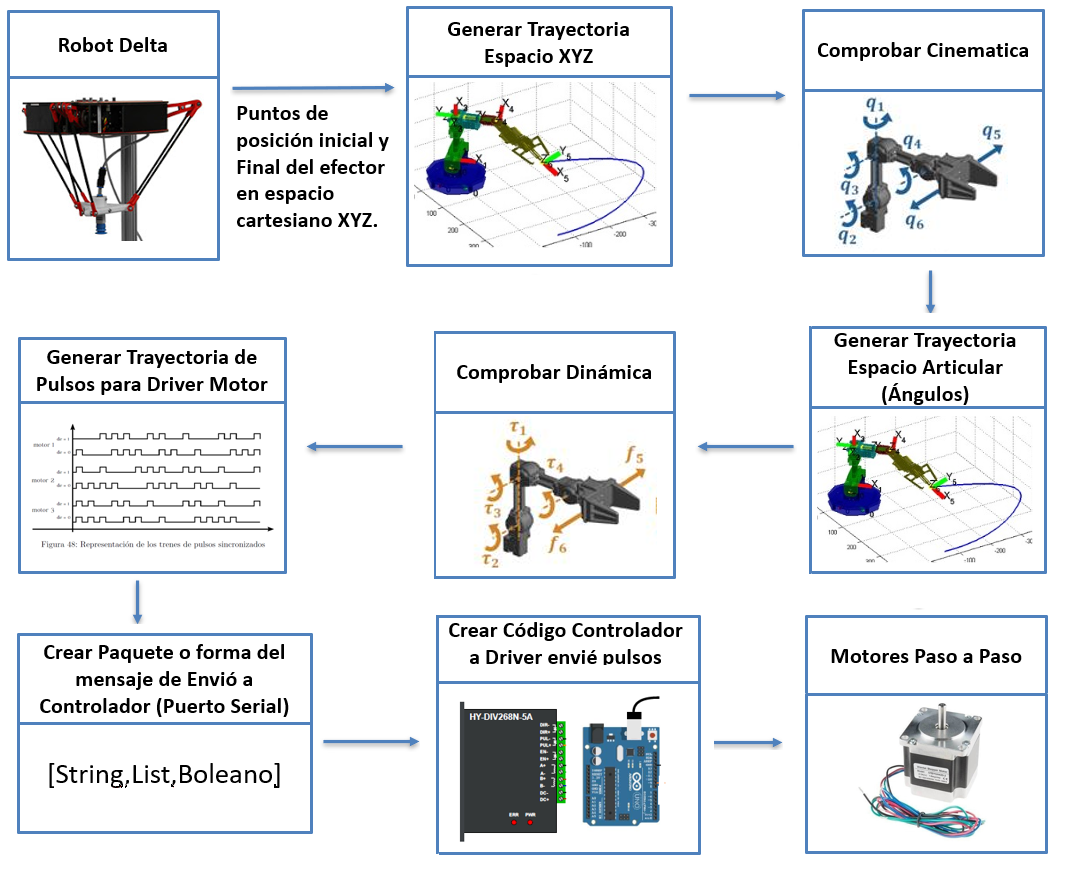
\includegraphics[width=0.8\linewidth]{Main/Chapter3/Images3/3-1/diagrama-de-flujo-robot.png}
        \caption{asd}
        \label{f:Cap3-1_diagrama_de_flujo_robot_accion}
    \end{figure}
    
Los pasos del diagrama de flujo son los siguientes:

\begin{enumerate}
    \item Definir los puntos de inicio y final de la trayectoria del robot.
    \item Elegir el tipo de trayectoria, posiciones, velocidades y aceleraciones impuestas y no dañar los componentes del robot.
    \item Comprobar la cinemática y dinámica para asegurar la trayectoria impuesta y no dañar los componentes del robot.
    \item Transformación de la trayectoria cartesiana al espacio articular de los actuadores que controlan el movimiento de las partes mecánicas del robot.
    \item Traducción de trayectoria en el espacio articular a pulsaciones que entiendan los drivers de cada motor.
    \item Envío de pulsos al driver de los motores por medio de un controlador.
\end{enumerate}

\section{Estructura de un robot delta}

    El robot delta puede ser subdivido por categorías de acuerdo al grupo estructural al que pertenezcan. Estas categorías facilitan la generación de conceptos para cada grupo de manera independiente \cite{Robot_parelelo_tipo}
    
    \begin{figure}[htb]
        \centering
        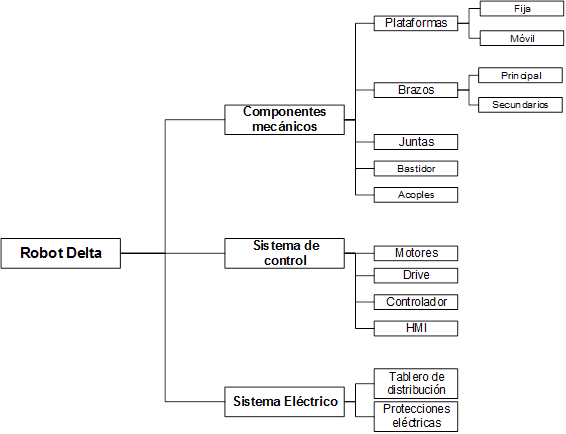
\includegraphics[width=1\linewidth]{Main/Chapter3/Images3/3-2/esquema-categorias-estructura.png}
        \caption{asd}
        \label{f:Cap3-2_esquema_arquitectura_robot_delta}
    \end{figure}
    
    Los componentes mecánicos son todas las piezas físicas que componen el robot delta. Es muy importante la elección del tipo de juntas a elegir ya que restringen el espacio de trabajo del robot delta. Por otro lado, se pueden optimizar las dimensiones de los largos de los brazos y antebrazos del robot con respecto a la energía suministrada a los motores y al espacio de trabajo.
    
    El sistema de control es todo lo que está relacionado con el control del movimiento del robot delta. Los motores, que mueven los brazos del robot delta, deben controlarse a través de drivers por la complejidad de su accionamiento. El controlador puede tener el algoritmo que cree las trayectorias cartesianas para realizar el movimiento del robot de un punto a otro. El HMI es la interfaz que ayuda a visualizar si el movimiento deseado del robot es correcto antes de que se realice.
    
    Los componentes eléctricos son todo lo relacionado con la electricidad como fuentes de poder para los motores, cables de conexión, fusibles, switch, etc.
    
    Con la intensión de modelar la arquitectura de un robot delta como guía para el desarrollo de este trabajo, se crea una arquitectura con ejemplos reales enfocado solo en el sistema de control, tal como se presenta en la figura \ref{f:Cap3-2_esquema_sistema_control} donde:
    
    \begin{itemize}
        \item \textbf{Software ROS:} Es el encargado de procesar y ejecutar los algoritmos de cinemática y dinámica del robot delta. Además, controla el envió, la recepción y el procesamiento de datos de los sensores y el controlador.
        \item \textbf{Controlador:} Realiza la conversión de la trayectoria cartesiana o angular a un formato compatible con el driver de los motores. Se puede utilizar Arduino, Raspberry Pi, etc.
        \item \textbf{Rviz:} Es la interfaz gráfica que simula las trayectorias del robot.
        \item \textbf{Kinect:} Sensor RGB y de profundidad que controla la posición del robot creando un lazo cerrado.
        \item \textbf{Actuadores:} Motores paso a paso controlados por drivers.
        \item \textbf{Encoder:} Sensor de velocidad y posición angular que controla los actuadores creando un lazo cerrado.
        \item \textbf{Gripper:} Pinzas qe sujetan los objetos.
    \end{itemize}
    
    Para controlar a un alto nivel cada punto anterior, se necesita de mucho estudio, investigación y práctica, por lo que en esta tesis solo abarcara lo relacionado con el Software ROS y la interfaz gráfica Rviz.  
    
    \begin{figure}[htb]
        \centering
        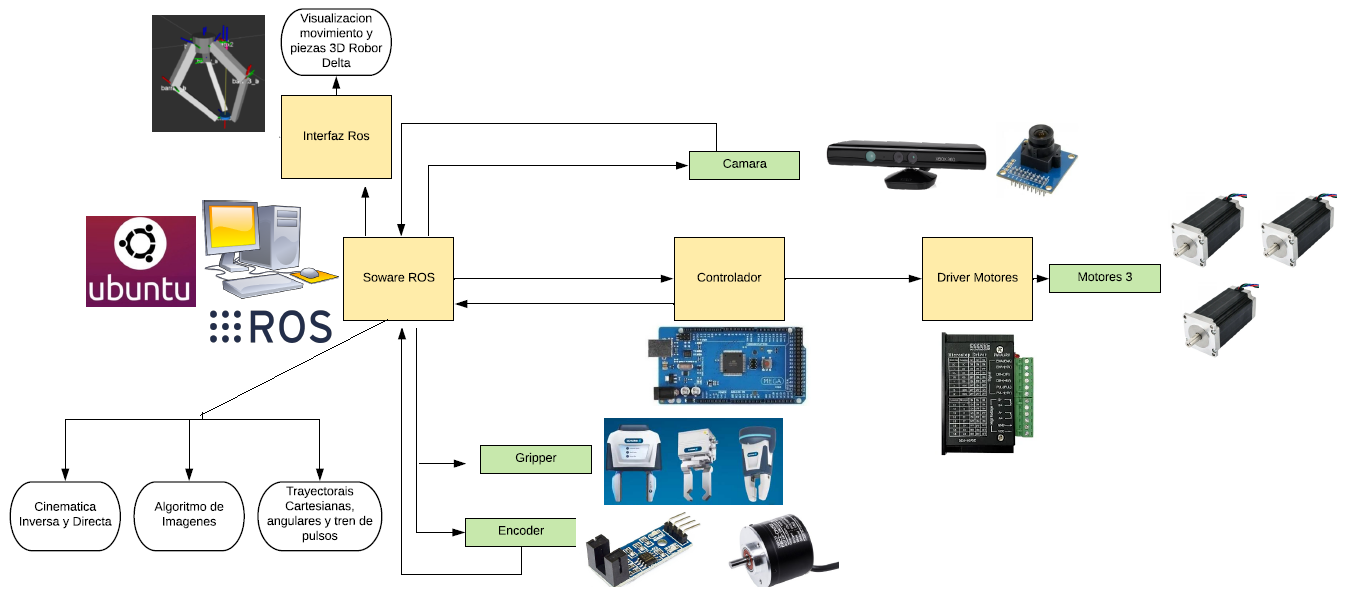
\includegraphics[width=1\linewidth]{Main/Chapter3/Images3/3-2/sistema-de-control.png}
        \caption{asd}
        \label{f:Cap3-2_esquema_sistema_control}
    \end{figure}
    
    

    
\section{Partes mecánicas (hay que repensar esto)}
    Con el fin de describir el robot delta, en esta sección se presenta un resumen del capítulo 2 de la tesis doctoral del ingeniero mecánico Reymond Clavel, el creador de este mecanismo, realizada en École Polytechnique Fédérale de Lausanne [referencia tanto]. 

    
    \subsection{Investigación}
    El primer objetivo que busca Reymond Clavel es el movimiento de piezas ligeras a gran velocidad en robots, ya que las aplicaciones objetivo de su investigación se encuentran en los campos del envasado en el sector alimentario, despaletización y paletización al inicio o al final de una línea de montaje, el montaje de componentes mecánicos, etc. Para todas estas operaciones se requiere un ritmo alto de producción/operación y los contactos de la industria de Clavel confirmaban esa tendencia en aquellos tiempos.
    
    Para lograr una alta tasa de trabajo durante operaciones que requieren carreras reducidas, el robot debe tener esencialmente una capacidad de aceleración y frenado; esta propiedad se obtiene mediante el uso de potentes actuadores debajo y mediante una estructura móvil muy ligera. Un estudio anterior de robot rápido del Clavel hizo posible probar el uso de gatos hidráulicos a alta velocidad con masas relativamente pesadas, pero por razones de coste y limpieza no querían utilizar energía hidráulica por lo que lo llevo al enfoque de una ``estructura móvil y ligera``.
    
    La búsqueda de un concepto se basó en una metodología enseñada en estudios de microtecnología en EPFL. Según la metodología antes mencionada, el primer paso de la cadena de costos consiste en definir la función global del producto considerado. La representación mediante una caja negra con las diferentes entradas y salidas sintetiza efectivamente esta información.
    
    \begin{figure}[htb]
        \centering
        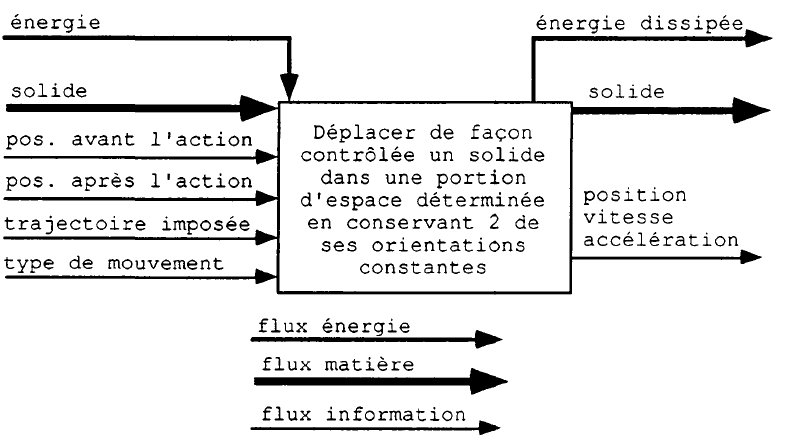
\includegraphics[width=1\linewidth]{Main/Chapter3/Images3/3-3/caja-negra-reymond.png}
        \caption{asd}
        \label{f:Cap3-3_caja_negra_reymond}
    \end{figure}
    
    
    
    \subsection{Elección del concepto ``Delta``}
    El catálogo de soluciones del anexo A2.2 de la tesis doctoral [tanto] presenta 18 tipos de soluciones principales que permiten mantener constantes 2 orientaciones de un sólido. La figura 2.3 muestra las soluciones más interesantes para el objetivo previsto. Entre estas 18 soluciones, Reymond conserva aquellas que tienen las siguientes particularidades:
    
    \begin{enumerate}
        \item El movimiento en el espacio (con tres grados de libertad) es proporcionado por el tres actuadores asegurados a la base fija, las soluciones 10 a 13 y 15 a 18 de la figura \ref{f:Cap3-3_soluciones_interesantes_catalogo} cumplen esta condición.
        \item Los actuadores son del tipo giratorio. Las soluciones 11, 13, 16 y 18 cumplen esta condicion.
        \item La estabilidad del órgano terminal está asegurada por una mayoría de elementos que trabajan en tensión-compresión más que en torsión. Finalmente se adopta la solución numero 18.
    \end{enumerate}
    
     \begin{figure}[htb]
        \centering
        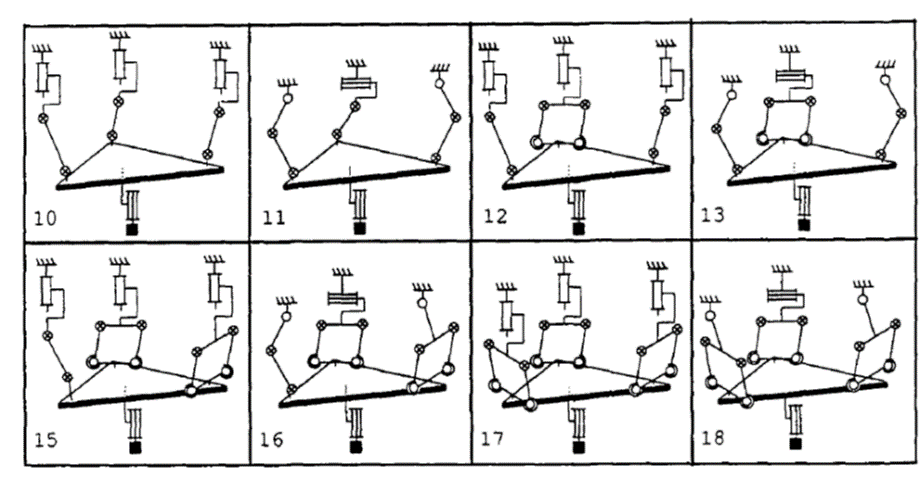
\includegraphics[width=1\linewidth]{Main/Chapter3/Images3/3-3/soluciones-interesantes.png}
        \caption{Extracto de las soluciones más interesantes del catálogo del Apéndice A.2.2}
        \label{f:Cap3-3_soluciones_interesantes_catalogo}
    \end{figure}
    
    \subsection{Descripción del concepto ``Delta'' y sus componentes}
    La figura \ref{f:Cap3-3_esquema_principal_robot_delta} sirve de apoyo para la descripción del robot DELTA y su funcionamiento. Este es un robot con cuatro grados de libertad. Se compone principalmente de una ``base fija'' (1) integrada a un marco de soporte de la instalación y una placa móvil (5); el nombre que se le da a esta última pieza es ``góndola'' (nacelle en frances). La conexión entre la base fija (1) y la góndola (5) se realiza mediante tres cadenas cinemáticas, cada una de ellas está formado por un ``brazo'' (2) montado en una articulación pivotante sobre la base fija y 2 ``barras paralelas'' (3) provistas cada una de una articulación (4) en cada extremo. El conjunto anterior que forma 2 barras paralelas y 2 elementos de conexión al brazo y a la góndola, se denomina ``paralelogramo''. Cada brazo (2) es impulsado por un ``motor de brazo'' (7) que, con mayor frecuencia, adopta la forma de un conjunto de motor reductor de sensor. La ``Pinza'' (10) del motor (6), a través del ``eje telescópico'' (8) provisto de una articulación tipo cardan (9) tiene oculto uno de sus extremos.
    
    \begin{figure}[htb]
        \centering
        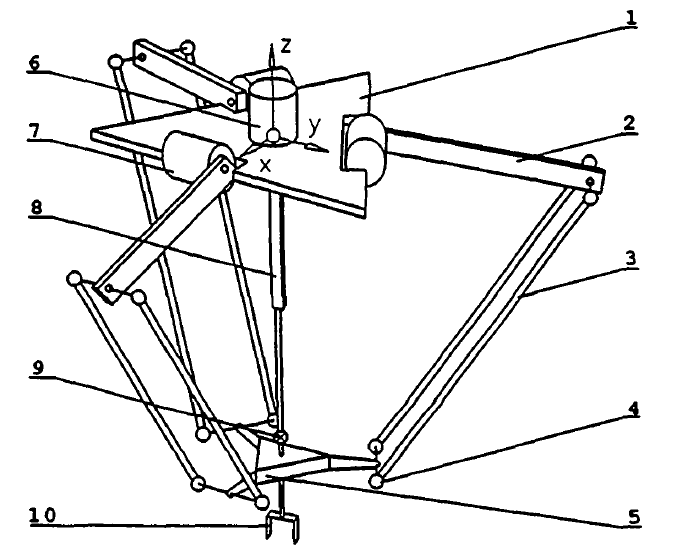
\includegraphics[width=0.5\linewidth]{Main/Chapter3/Images3/3-3/esquema-principal-robot-delta.png}
        \caption{Esquema principal del robot delta}
        \label{f:Cap3-3_esquema_principal_robot_delta}
    \end{figure}
    
    La orientación de la góndola está asegurada constantemente por los 3 paralelogramos que comprenden cada uno 2 dimensiones pequeñas y 2 dimensiones grandes formadas por las barras paralelas. Cada lado pequeño integrado al extremo de un brazo permanece constantemente paralelo al eje de rotación del brazo en cuestión. Los 3 pares de barras paralelas aseguran que las 3 pequeñas dimensiones integradas a la góndola permanezcan paralelas a las pequeñas dimensiones integradas a los extremos de los brazos, por tanto, paralelas a los ejes de rotación de los brazos que, por construcción, se ubican en el mismo plano. Las juntas en los extremos de las barras paralelas son del tipo de junta esférica, por lo que cada barra puede girar alrededor de su eje longitudinal; esta rotación no altera el comportamiento de esta estructura articulada que forma el paralelogramo del espacio. Una conexión por resortes y estribos entre las 2 barras paralelas simplifica la construcción de las rótulas y limita las evoluciones giratorias de las barras paralelas.
    
    \begin{figure}[htb]
        \centering
        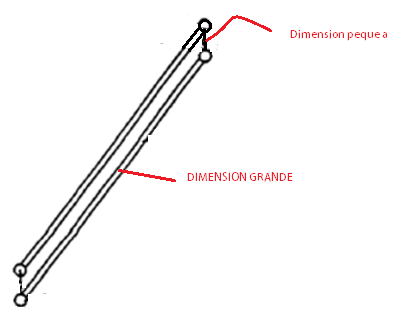
\includegraphics[width=0.5\linewidth]{Main/Chapter3/Images3/3-3/ayuda-dimensiones.png}
        \caption{Representación de uno de los ``paralelogramos'' del robot delta}
        \label{f:Cap3-3_ayuda_dimensiones}
    \end{figure}
    
    
\section{Software Robor Operating System (ROS)}
    Desde
    \subsection{Arquitectura y conceptos}
        Desde
    \subsection{Herramientas y librerías}
        Desde

\section{Interfaz de visualización (Rviz)}
    Desde
    
\section{Software Algorithm Development and mining (ADAMS)}
Desde

    
      
        
            
            
            

        
    
    